\section{Cherenkov Radiation}
\label{ch:cherenkov_radtion}
When a charged particle travels through a material at a speed faster than the phase velocity of light in the material, Cherenkov radiation is produced.  Molecules excited by the particle release light, and when the particle is traveling faster than $c/n$, the light emitted from different points along the particles path interferes constructively to create Cherenkov radiation, as shown in \cref{fig:cherenkovradiation}.  The requirement for Cherenkov radiation is thus
\begin{equation}
\beta>\frac{1}{n}.
\label{eq:cherenkov_req}
\end{equation}
The Cherenkov radiation is emitted from the path of the charged particle along a cone centered on the path of the charged particle with half opening angle $\theta_C$ given by:
\begin{equation}
\cos \theta_C=\frac{1}{\beta n}.
\label{eq:cherenkov_angle}
\end{equation}
A detailed derivation of these formula based on electrodynamics can be found in \cite{Jackson:1998nia}.
\begin{figure}
\centering
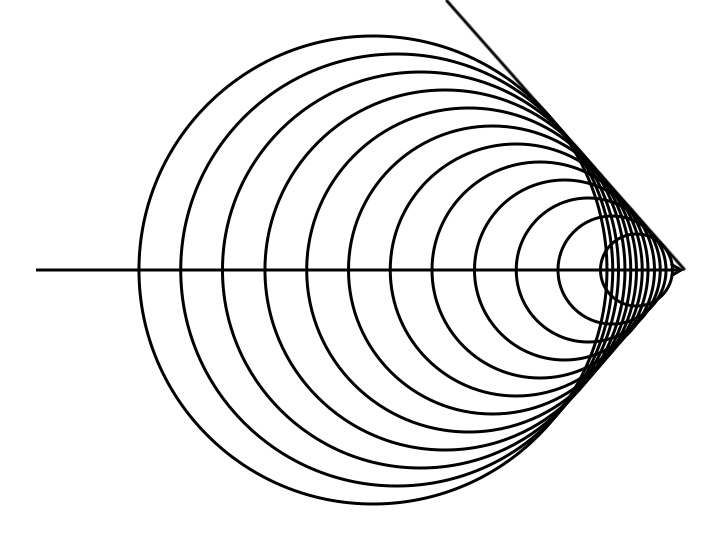
\includegraphics[width=0.8\textwidth]{figures/Cherenkov_radiation.png}
\caption{Constructive interference resulting in Cherenkov radiation.}
\label{fig:cherenkovradiation}
\end{figure}
The index of refraction of water is 1.34, so for charged particles in water the cherenkov threshold corresponds to $\beta>0.75$.  This can be translated to a momentum threshold of $p>1.13m$, which equates to a momentum threshold of 577 KeV/c for electrons, 119 MeV/c for muons, 157 MeV/c for charged pions, and 1.058 GeV/c for protons.  The cherenkov angle for a highly relativistic charge particle in water ($\gamma \gg 1$) of about 42$^\circ$.  \par
The emitted spectrum is described by the formula\cite{Olive:2016xmw}:
 \begin{equation}
\frac{d^2N}{d\lambda dx}=\frac{2\pi \alpha z^2}{\lambda^2}\left(1-\frac{1}{\beta^2\n^2(\lambda)}\right)
\label{eq:cherenkov_spectrum}
\end{equation}
where $\alpha$ is the fine structure constant, $z$ is the charge of the particle (in units of electron charge), $\lambda$ is the wavelength of the emitted light, and $x$ is the distance traveled by the charged particle.  It should be noted that whil this formula allows for a wavelength dependent index of refraction, the index of refraction of water is quite stable of the range of wavelengths observed by PMTs.   
